\chapter{Results and Discussion}\label{result_chapter}
In this chapter result of two different method are given. First section contain the results of classical methods while in second second section Bayesian analysis was performed.
\section{Classical approches analysis}
In this section Combine ANOVA, AMMI model,Cluster analysis  and GGE biplot methods are applied for the diagnosis of wheat crop data which comprises of 30 genotypes tested at 13 locations for two year. 
\subsection{Combined Analysis of Variance}
The combined analysis of variance (ANOVA) of thirty genotypes in 13 environment for 2 years was performed and output is provided in (Table~\ref{Table:4.1}). Analysis showed that genotype and environment were highly significant, which mean these effect have significant differences among them (p<0.01). Significance of G$\times$E interaction (p<0.01) indicated that genotypes have different responses in different environments. Environment, genotypes  and G$\times$E explained 84.3\%, 3.5\% and 8.6 \% variation of sum of square. 

\begin{table}[h!]
\centering	
\caption[Combined Aanlysis of Variance]{Combined analysis of variance (ANOVA)  }
\label{Table:4.1}
\begin{tabular}{l r r r r r}
	\toprule\hline
	
	Sources & DF & SS & MS & p-value & \% Sum of square   \\\hline
	\midrule
	Environment (E) & 25  & 2226401709 & 89056068 & 0.00 & 84.3   \\
	Rep(ENV)        & 52  & 3653099    &  70252   & 0.1861 & \\
	Geneotype (G)   & 29  & 92402025   & 3186277  & 0.00  & 3.5 \\
	G$\times$E      & 725 &  227172934 &  313342  & 0.00 & 8.6  \\ 

	Residual        & 1508& 90129189   &  59767   &        & \\ 
	\bottomrule\hline
	
\end{tabular}

\end{table}

From Combined ANOVA provided in (Table~\ref{Table:4.1}), it is evident that G$\times$E have significant effect hence the identification of superior genotypes across environment is not possible on the basis of just performance of mean yield. Furthermore, ANOVA unable to partition the interaction in various component, so other stability measures are required for to explore G$\times$E.

\subsection{AMMI analysis and bi-plot representation}
As (Table~\ref{Table:4.1}) indicated  that main effect as well as interaction effect were significant, so G$\times$E is partitioned into bilinear terms. The IPCA are arrange in ascending order on their importance give in table (Table~\ref{Table:4.2}).  G$\times$E  interaction component significance was measure using the Gollob's F-test at 0.01 probability. First four principal components explained 59.2\% variation of GEI sum of squares. Hence, AMMI-4 model can be regarded as best fit model for the wheat crop data. 
 
 \begin{table}[h!]
	\caption[Combined analysis of variance (ANOVA) according to the AMMI]{Combined analysis of variance (ANOVA) according to the AMMI model and Gollob's test of interaction PC's  } 
	
	\label{Table:4.2}
	%\centering  % not needed, since table is as wide as text block
	\begin{tabular}{l r r r r r r}
		\toprule\hline
	 
	Sources                 & DF  & SS         & MS & p-value & G$\times$E (\%) & Cumulative(\%) \\
	\hline	\midrule
			Environment (E) & 25  & 2226401709 & 89056068 &            &  &\\
			Rep(ENV)        & 52  & 3653099    &  70252   &            &  &\\
			Geneotype (G)   & 29  & 92402025   & 3186277  &            &  & \\
			G$\times$E      & 725 &  227172934 &  313342  &            &  &\\ 
\multicolumn{1}{r}{	IPCA 1} & 53  & 53024110   & 1000455  & 0.00       & 23.3 & 23.3 \\
\multicolumn{1}{r}{IPCA 2}  & 51  & 31803670   & 623601   & 0.00       & 14.0 & 37.3 \\
\multicolumn{1}{r}{IPCA 3}  & 49  & 27472720   &  560667  & 0.00       & 12.1 & 49.4 \\
\multicolumn{1}{r}{IPCA 4}  & 47  & 22299260   & 474452   & 0.00       & 9.8  & 59.2 \\
\multicolumn{1}{r}{IPCA Residual}   & 525 &    92573174   & 176329.8   &  0.00  & & \\
			Residual        & 1508& 90129189   &  59767   &        & & \\ 
		\bottomrule \hline
		
	\end{tabular}
	IPCA = Interaction Principal Component Axis
\end{table}
Although, first four component were found significant, but to avoid from complexity first two principal component can be used to analyze result using AMMI biplot. For predictive model two principal components for interaction were adequate. Whereas, other components mostly contain the non-predictive variation. Therefore, the interaction of thirty genotypes of wheat along with 26 environments  was by first two component, as \cite{KAYA2002} suggested that predictive criterion choose such model which  consist of two interaction principal components.

First IPC axis explained 23.3\% variation while 14.0\% was captured by the second principal component for interaction sum of square.  First two PC cumulatively explain 37.3\% variation for interaction sum of squares with 104 degree of freedom out of 725  was an indication that sufficient percentage of G$\times$E explained. So further diagnosis can be done by graphing a biplot using first two IPCA. 

\subsubsection{AMMI bi-plot}
The biplot of PCA-1 versus the PC1-2 containing 37.3\% variation is displayed in (Figure~\ref{Figure:4.1 }). Important information related to the interaction can obtained from the direction of genotypes and environments. From plot, it can be observe that  11BT004  has a positive interaction with S10(Vehari-14) and L10(Vehari-13) and a negative interaction with S13(Piplan-14) and S13(piplan-13). Genotypes NR-411, 11BT004 and V-12304 having high PC1 and PC2 score shown that they have significant effect in interaction.
\begin{figure} [h!]
	\centering  
	\scalebox{0.40}
	{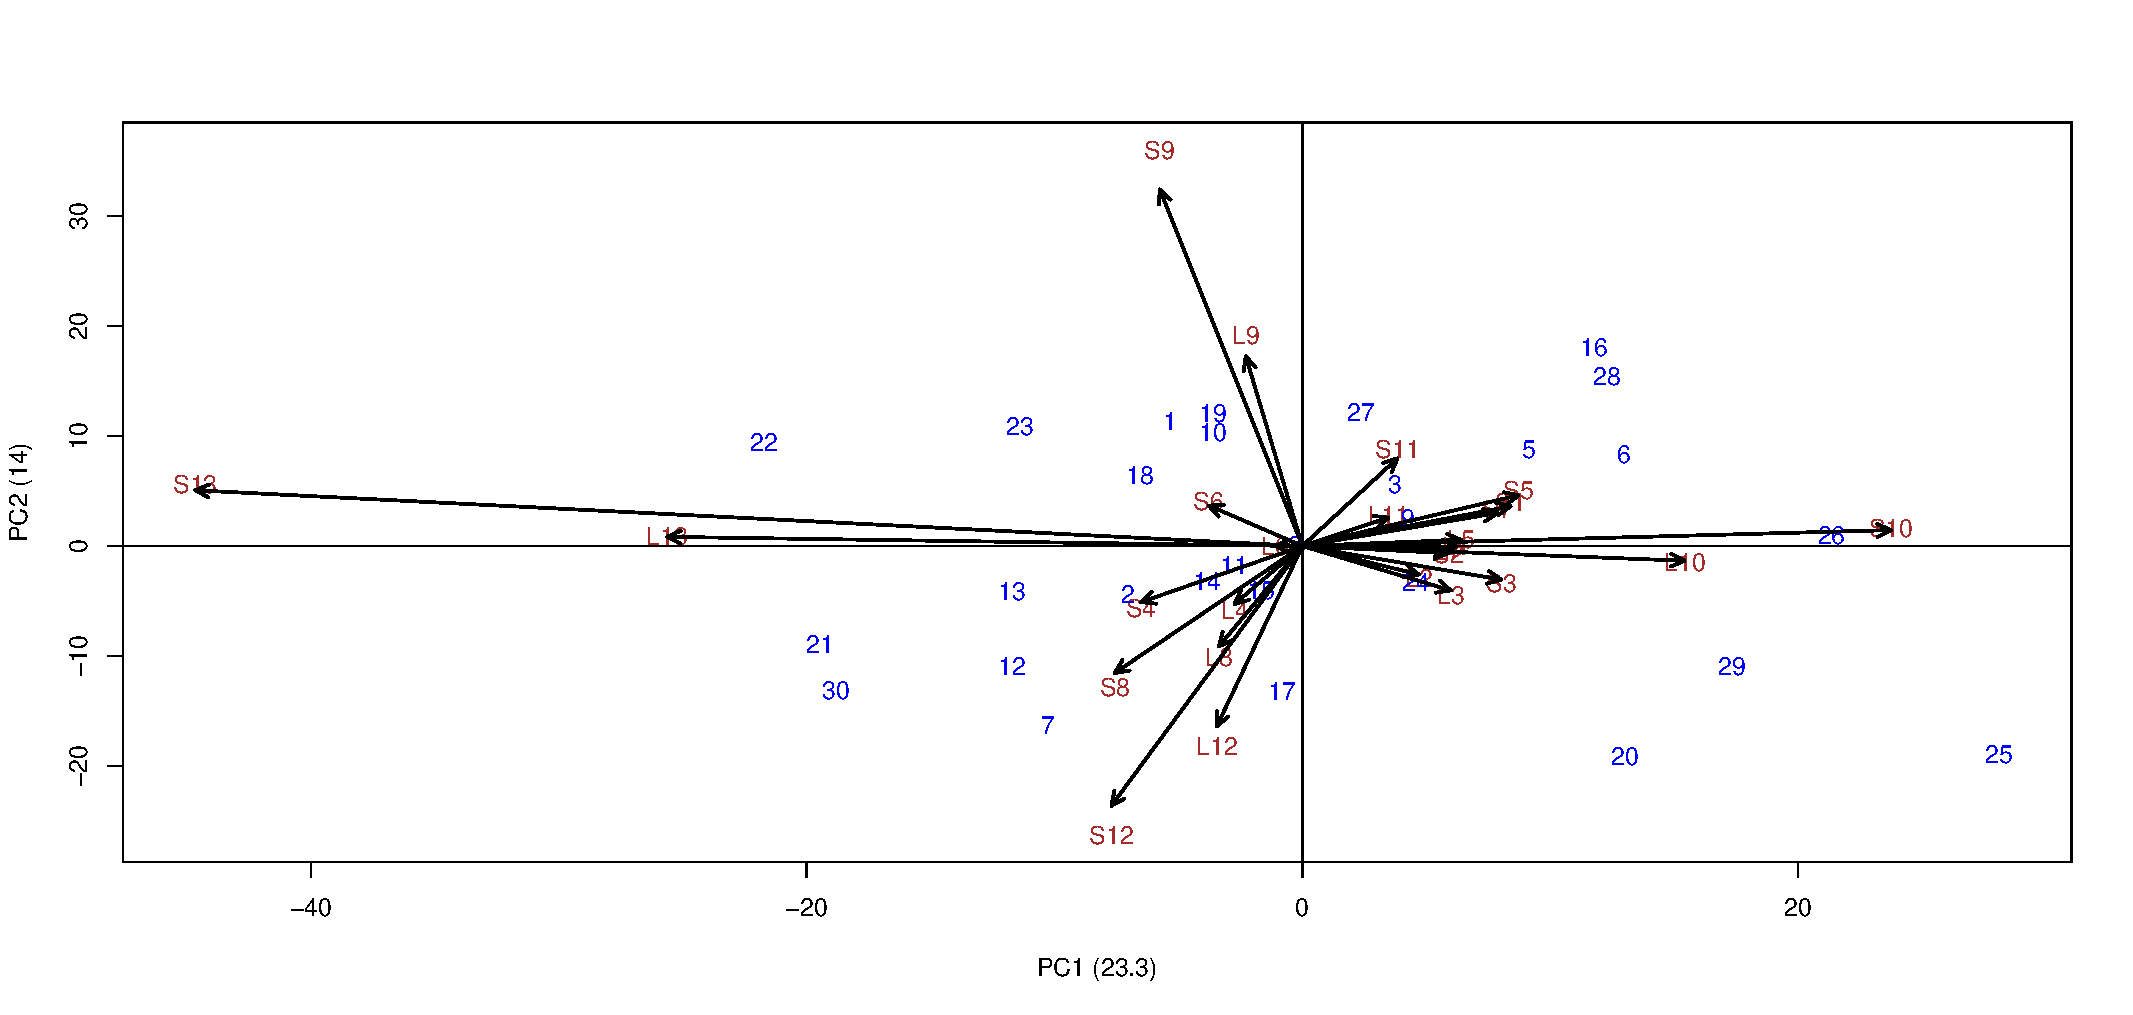
\includegraphics[width=14in,height=12in]{02ThesisMain/Ch04RD/figures/k.pdf}}
	\caption[Biplot of IPCA axis-1 versus Axis-2]{ Biplot of interaction principal component analysis (PCA) axis-1 versus axis-2 of wheat data for 30 genotypes in 26 environments  }
	\label{Figure:4.1 }
\end{figure}
\clearpage
The second biplot was of IPCA axis-1 versus the mean yield of environments and genotypes [Figure\ref{Figure:4.2 }]. The low yielding genotypes were located in upper left  and environments are shown in lower left quadrant. Among environments; S4(BWN-14), S9(Multan-14) and S10(Vehari-14) were higher yielding environments, whereas  S13(Piplan-14) and S8(Khanewal-14) were the most favorable environments. Among 26 environments L6( Gujranwala-13) was low yielding and was the most unfavorable environment. 
\begin{figure} [h!]
	\centering  
	\scalebox{0.4}
	{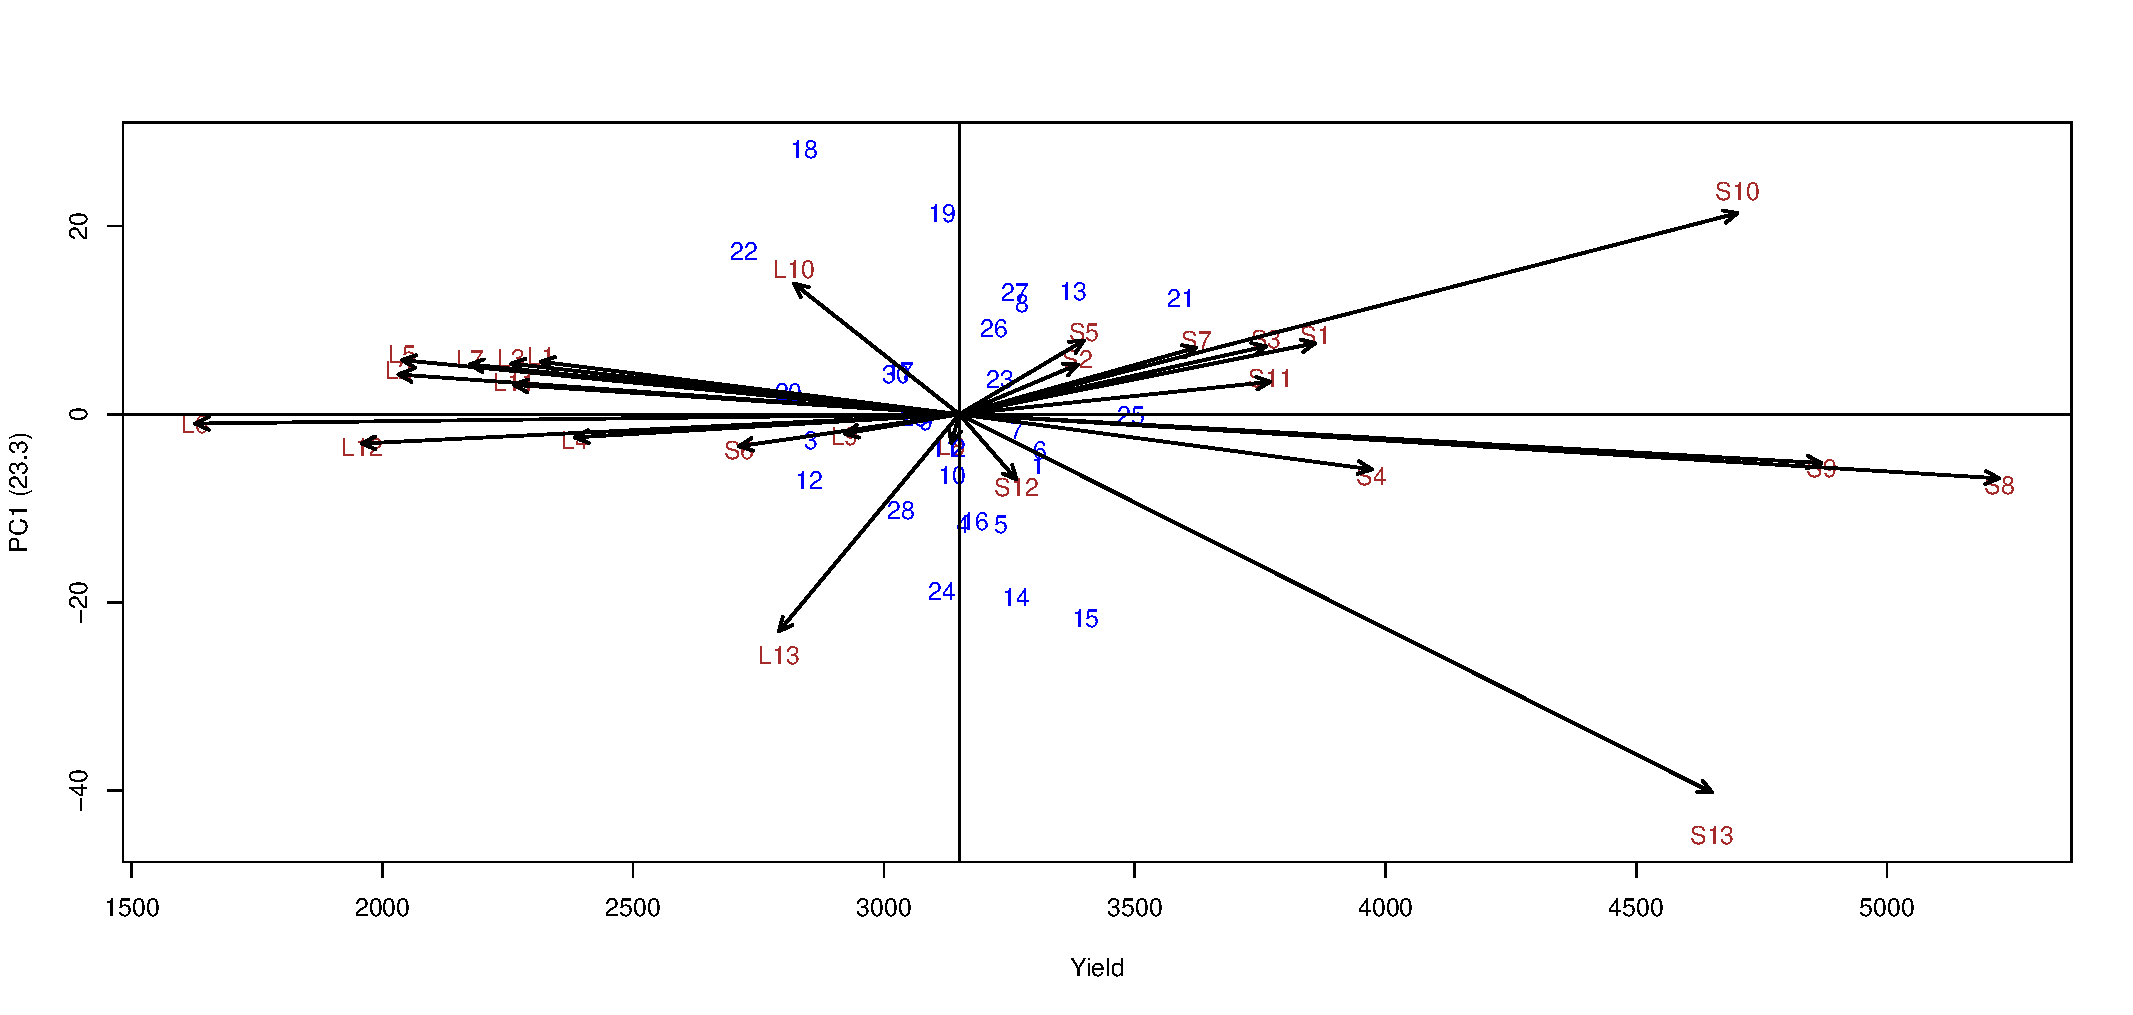
\includegraphics[width=15in,height=14in]{02ThesisMain/Ch04RD/figures/myplot}}
	\caption[Biplot of IPCA axis-1 versus mean yield]{Biplot of interaction principal component analysis (PCA) axis-1 versus mean yield of wheat data for 30 genotypes in 26 environments  }
	\label{Figure:4.2 }
\end{figure}

\clearpage    
\subsubsection{AMMI Stability Value (ASV)}
ASV is the distance from zero in a two dimensional scatter-gram of IPCA1 scores against IPCA2 scores. As in GEI the contribution of PC-1 is much more than that of PC-2, so more weight was give according to the relative contribution of PC's \citep{Farshadfar2008}. The distance from zero was obtain by applying Pythagoras theory \citep{Purchase1997}.
\begin{table}[h!]
	\centering
	\caption[AMMI stability values]{Mean yield genotypes, scores for the IPC 1 and IPC 2, AMMI stability (value ASV), rank of genotypes based on ASV and genotype  selection index for 30 genotypes } 
	\label{Table:4.3}
\begin{tabular}{l r r r r r} 
		\toprule \hline
   Genotype & Mean yield ($Y_i$) & Rank ($Y_i$) & ASV & Rank of ASV & GSI\\ 
	\midrule \hline



		
	V-12266  & 3307.80 & 6  & 13.32 & 15 & 21 \\
	V-11047  & 2850.33 & 27 & 10.11 & 9  & 36 \\
	V-12284  & 3230.41 & 12 & 7.41  & 8  & 20\\
	V-11098  & 3493.20 & 2  & 0.22  & 1  &  3\\
	V-11061  & 3218.96 & 13 & 14.68 & 16 &  29 \\
	V-11022  & 3261.07 & 10 & 18.67 & 20 & 30   \\
	V-11092  & 3032.99 & 23 & 21.00 & 21 & 44   \\
NW.10.1111-7 & 3059.22 & 22 & 0.41  & 2  & 24  \\
	TW11510  & 3023.16 & 25 & 6.03  & 6  & 31  \\
	V-12275  & 3148.69 & 16 & 11.32 & 11 & 27 \\ 
	GH       & 2853.74 & 26 & 3.98  & 3  & 29 \\
	V-11137  & 3157.16 & 15 & 18.65 & 19 & 34 \\
	NN-GAN-3 & 3232.26 & 11 & 15.69 & 17 & 28 \\
	V-11138  & 3310.37 & 5  & 5.89  & 5  & 10 \\
	V-11046  & 3264.55 & 8  & 4.61  & 4  & 22 \\
	NR-411   & 3274.53 & 7  & 23.61 & 23 & 30 \\
	V-11365  & 3084.32 & 21 & 13.28 & 14 & 35 \\
	V-12265  & 3135.73 & 17 & 10.62 & 10 & 27 \\
	Millat-11& 3121.67 & 18 & 12.90 & 13 & 31 \\
Lasani-08    & 3376.89 & 4  & 25.43 & 25 & 29 \\
	Nr-409   & 3262.65 & 9  & 26.66 & 26 & 35 \\
	V-11143  & 3401.76 & 3  & 29.60 & 29 & 32 \\ 
	V-11041  & 3181.39 & 14 & 18.28 & 18 & 32 \\
	V-11032  & 3031.73 & 24 & 6.77  & 7  & 31 \\
	NS-10    & 2839.56 & 28 & 40.95 & 30 & 58 \\
	11BT004  & 3115.61 & 20 & 27.57 & 27 & 47 \\
	9459-1   & 2809.60 & 29 & 12.54 & 12 & 41 \\
	V-12304  & 3591.69 & 1  & 12.54 & 22 & 23 \\
	11B2074  & 2720.89 & 30 & 24.91 & 24 & 24 \\
	11B2049  & 3116.34 & 19 & 27.58 & 28 & 47 \\
	 \bottomrule\hline
\end{tabular}
\end{table} 

AMMI stability value, mean and genotype selection index are given in (Table \ref{Table:4.3}). Stability analysis showed that mean yield  have range from 2720.9 to 3591.69 kg/plot and ASV ranged from 0.22-40.95 for wheat genotypes. In ASV as V-11098  followed by , NW.10.1111-7 and "GH" gave the lowest ASV values indicated these were the most stable genotypes, while NS-10 was recognized the most unstable as it gave the highest ASV.
\subsubsection{Genotype selection index (GSI)}
It is not necessary that stable genotype also give the highest yield  so stability per \textit{Se} should not be only selection parameter. As ASV take into account both stability and yield criteria , so according to ASV given in (Table \ref{Table:4.3}) V-11098  was chosen as the most desirable genotype for selection based on  stability high yielding performance; whereas, NS-10 having highest GSI was least desirable. 

\subsection{GGE-biplot}
Visual results using GGE biplot  of 30 wheat genotypes in 26 different environments are plotted in Figures 4.3 to 4.8. GGE analysis Revealed that, IPCA 1 explained 33.91\% of G$\times$E variation, where as G+GE variation was explained by IPCA2 was 16.02\%. Over all GGE biplot explained 49.93\% by both axis.

In [Fig.\ref{Figure:4.3}] GGE-biplot based on genotype focused scaling is represented for the identification where the genotypes are located. The genotypes V-12304, V-11143, Nr-409, NR-411,  Lasani, V-11022 , V-11061 , V-11098, gen-14, V-12266  were above average, while  other genotypes were below average. These above average genotypes can be divided into two groups;  V-12266, V-11138,  V-11046, and V-11098 were declared stable because they have low PC2 score and others were considered unstable genotypes (having high PC2 score).

\begin{figure} [h!]
	\centering  
	\scalebox{0.3}
	{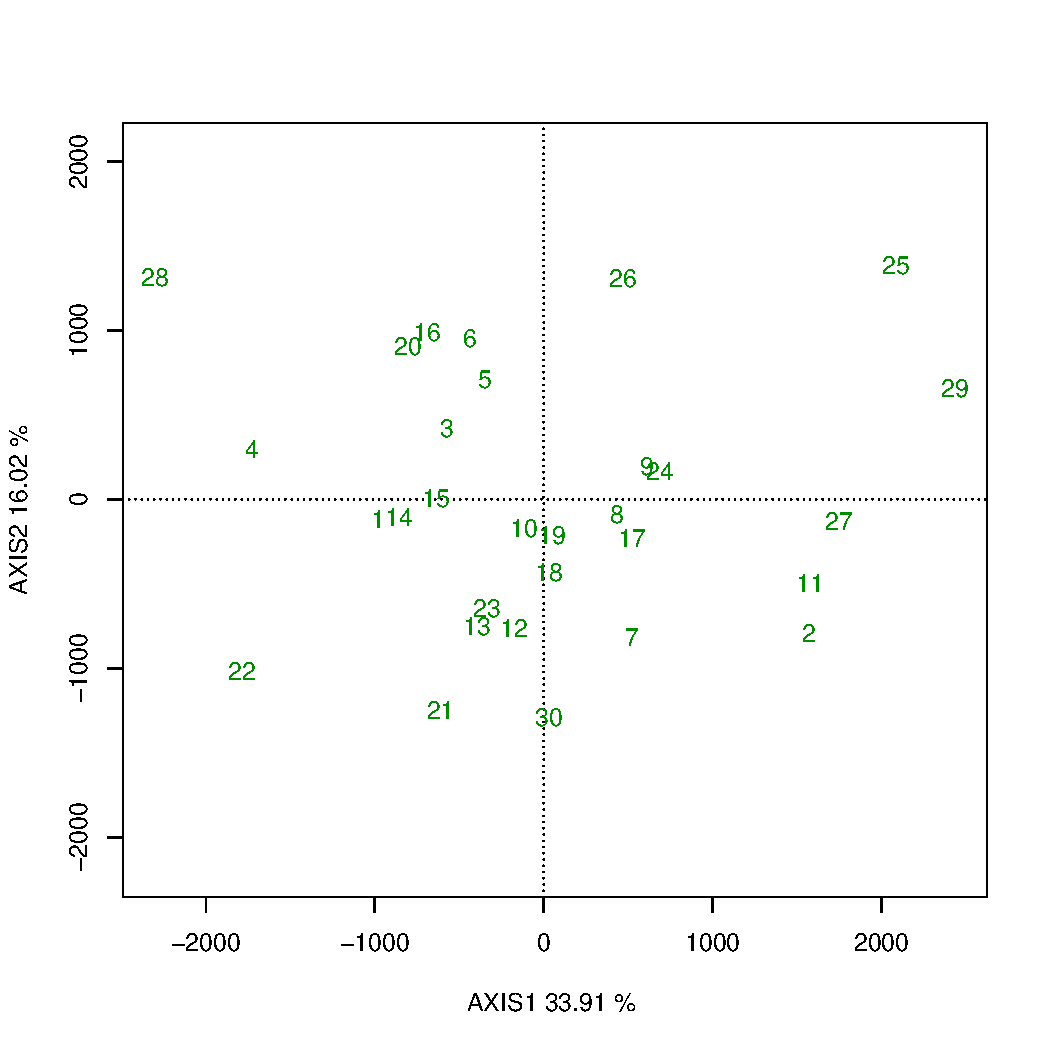
\includegraphics[width=410mm]{02ThesisMain/Ch04RD/figures/gfscale}}
	\caption[GGE-biplot based on genotype-focused scaling for genotypes]{GGE-biplot based on genotype-focused scaling for genotypes. Details of genotypes are give in Table 3.1 }
\label{Figure:4.3}
\end{figure}



GGE Biplot  based on environment-focused scaling was plotted to explore relationship among environments, it was shown that all environment exhibited similar direction with respect to PC 1. The angles between  environments shown that, they can be divided in four mega environments. S10( Vehari-13) ans L10( Vehari-13) formed a group [Fig.\ref{Figure:4.4}], while S12(Sargodha-14), L12(Sargodha-13), S13(Piplan-14) and L13(Piplan13) formed other one. remaining genotypes further were grouped in two mega-environments. Standard deviation related within environments can be approximated by the length of vector. Among 26 environments S13(Piplan-14) and S10(Vehari-13) were found most discriminant environments, where as, L12(Sargodha-13) and L6(Gujranwala-13) were least discriminant among all environments. 

\begin{figure} [H]
	\centering  
	\scalebox{0.3}
	{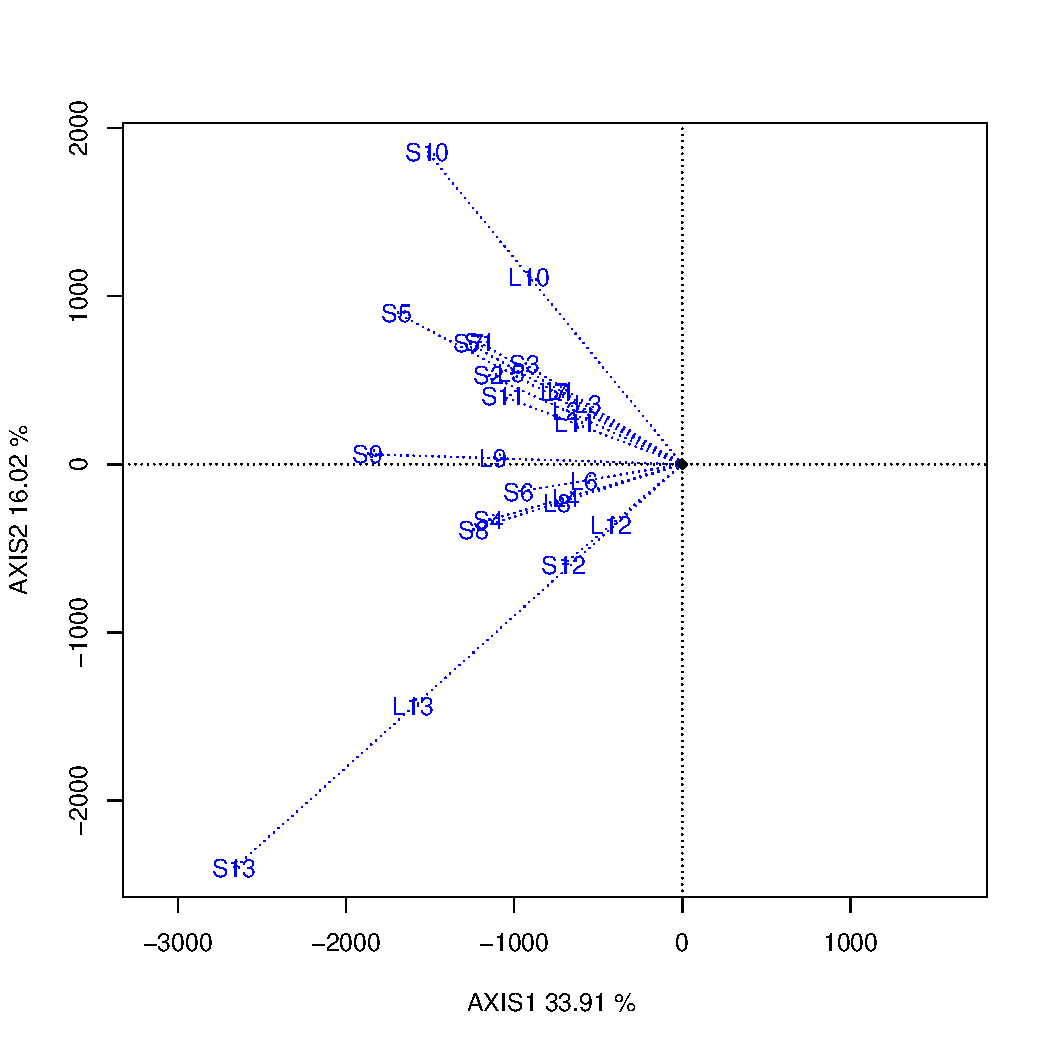
\includegraphics[width=460mm]{02ThesisMain/Ch04RD/figures/efscale}}
	\caption[GGE-biplot based on environment-focused scaling for environments]{GGE-biplot based on environment-focused scaling for environments. Details of environments are give in Table 3.2}
\label{Figure:4.4}
\end{figure}



To assess where the genotypes is best suited, genotypes were plotted against environments for the visualization of which-won-where pattern [Fig.\ref{Figure:4.5}]. In this biplot, a polygon was formed by joining the six vertex of genotypes V-12304, NS-10,  11B2074, V-11047, 11B2049 and V-11143; which were the most responsive genotypes. Corners also gave the idea that  Genotype V-11143 and  V-12304 were low yielding. From the polygon view  were close to ideal genotypes suggested by \cite{Yan2005}. 

\begin{figure} [H]
	\centering  
	\scalebox{0.3}
	{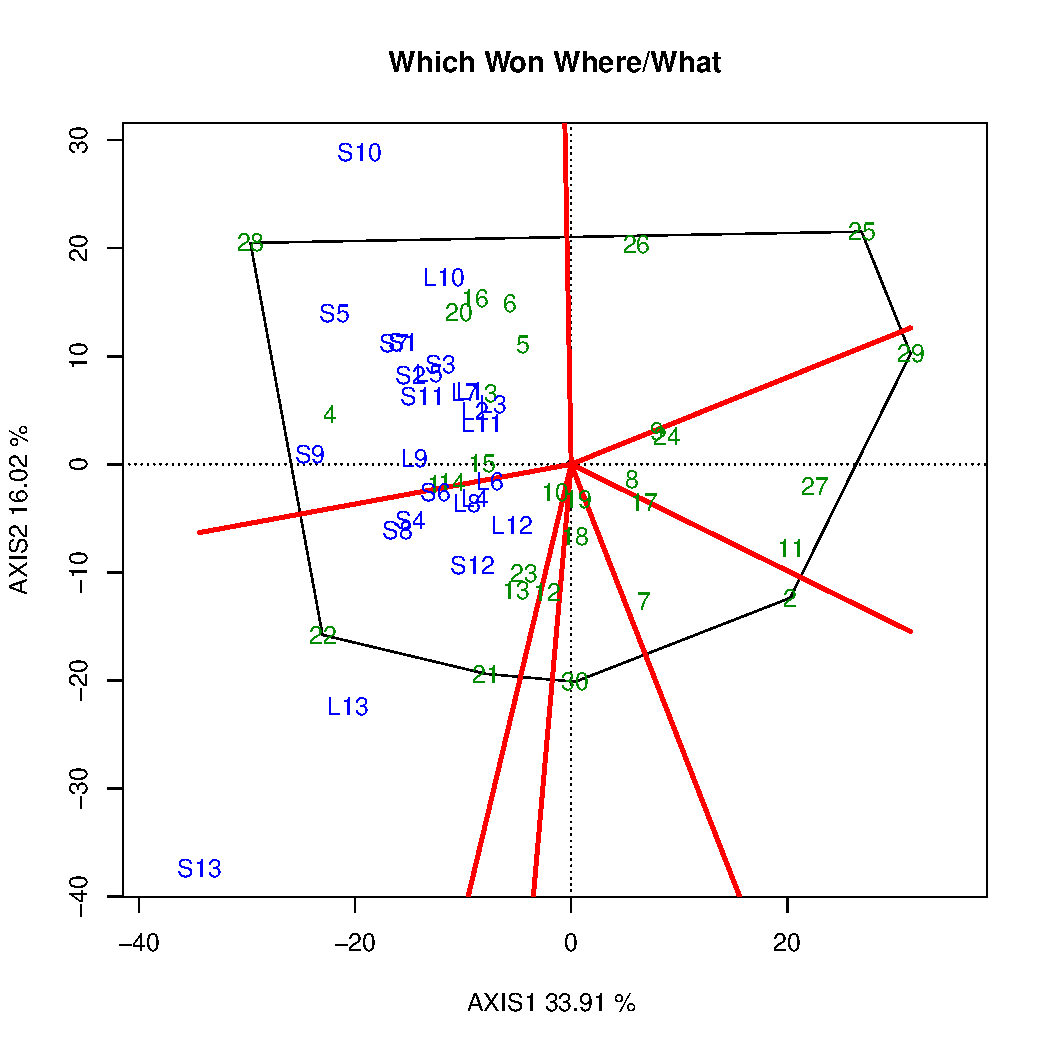
\includegraphics[width=460mm]{02ThesisMain/Ch04RD/figures/www}}
	\caption[Polygon views of GGE-biplot based on symmetrical scaling]{Polygon views of GGE-biplot based on symmetrical scaling for the which-won-where pattern for genotypes and environments}
\label{Figure:4.5}
\end{figure}




A GGE biplot viewing the Average environment coordination (AEC) based on genotype focused scaling is portrayed in [Fig.\ref{Figure:4.6}]. The average-environment axis (AEA) points to higher average seed yield; while average-environment coordinate (AEC) which is perpendicular to AEA points to greater variability in either direction. Results revealed that 11B2074 have the highest yield where as V-12304 gave the lowest. Genotypes; V-11143, NS-10, 11BT004 and 11B2049 having large AEC projection indicated that these were least stable and genotypes V-11098, V-11047, NW.10.1111-7, V-11046,  GH,  V-11365 and 9459-1 were proved to be most stable. Hence on basis of both mean yield and stability genotypes 9459-1, NW.10.1111-7, GH, V-11047 were recommended as the most favorable genotypes.      

\begin{figure} [H]
	\centering  
	\scalebox{0.3}
	{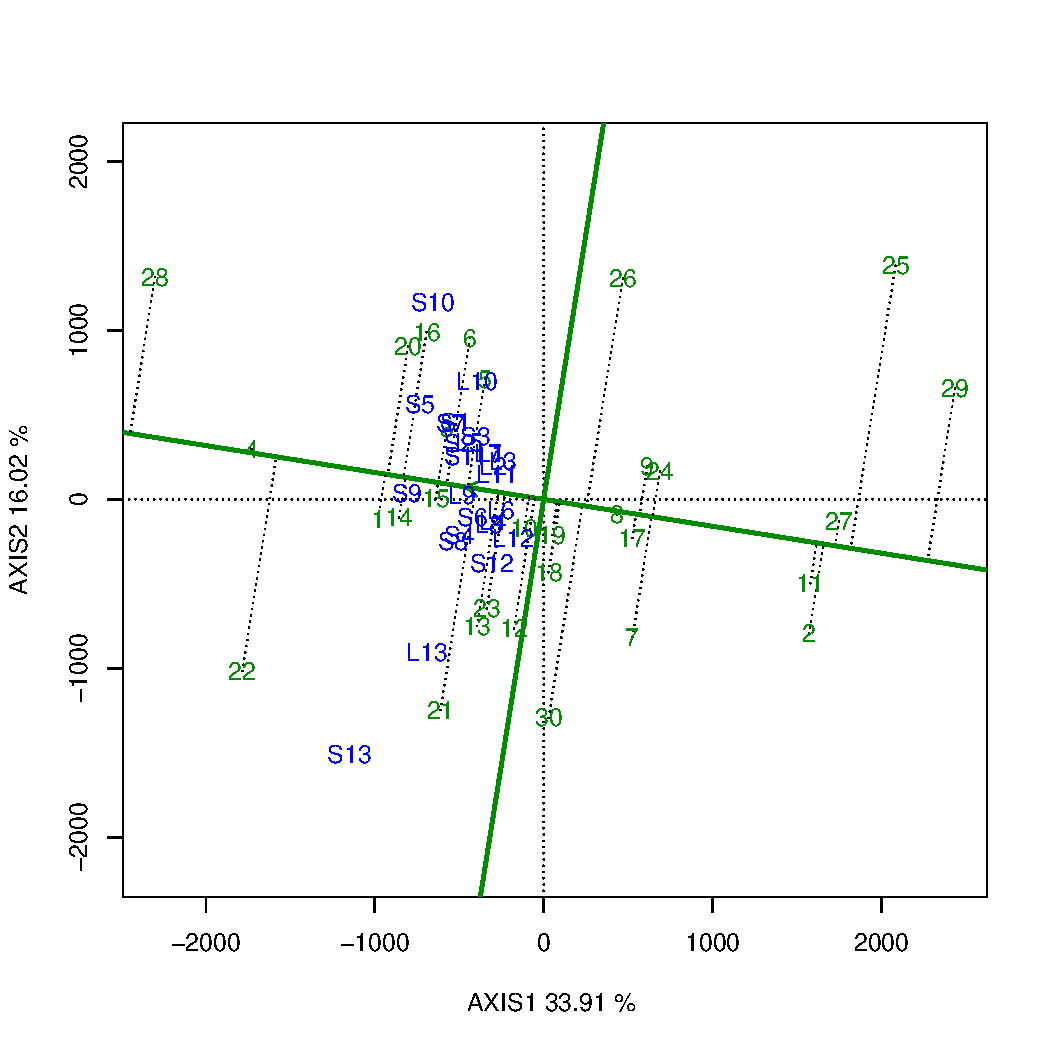
\includegraphics[width=460mm]{02ThesisMain/Ch04RD/figures/AEC}}
	\caption[Average environment coordination (AEC) views of the GGE-biplot]{Average environment coordination (AEC) views of the GGE-biplot based on gen-focused scaling for mean performance and the stability of genotypes}
\label{Figure:4.6}
\end{figure}



GGE biplot also facilitate in assessment of ideal genotype showing concentric circles, as \citep{Farshadfar2008} suggested ideal genotype (high mean yield and the most stable one) should be located in the center. No genotype was located in center [Fig.\ref{Figure:4.7}], so V-11098 was considered as the most desirable genotype across all environments as it lie on first concentric circle as The closer a genotype to the ideal one is the more valuable it is. Although such an "ideal" genotype may not exist in reality, it can be used as a reference for genotype evaluation \citep{Yan2005}. Genotypes  11B2074 and NS-10 although gave the high yield located at far away from center so these were recommended the most  undesirable genotypes among all genotypes. 
\begin{figure} [H]
	\centering  
	\scalebox{0.3}
	{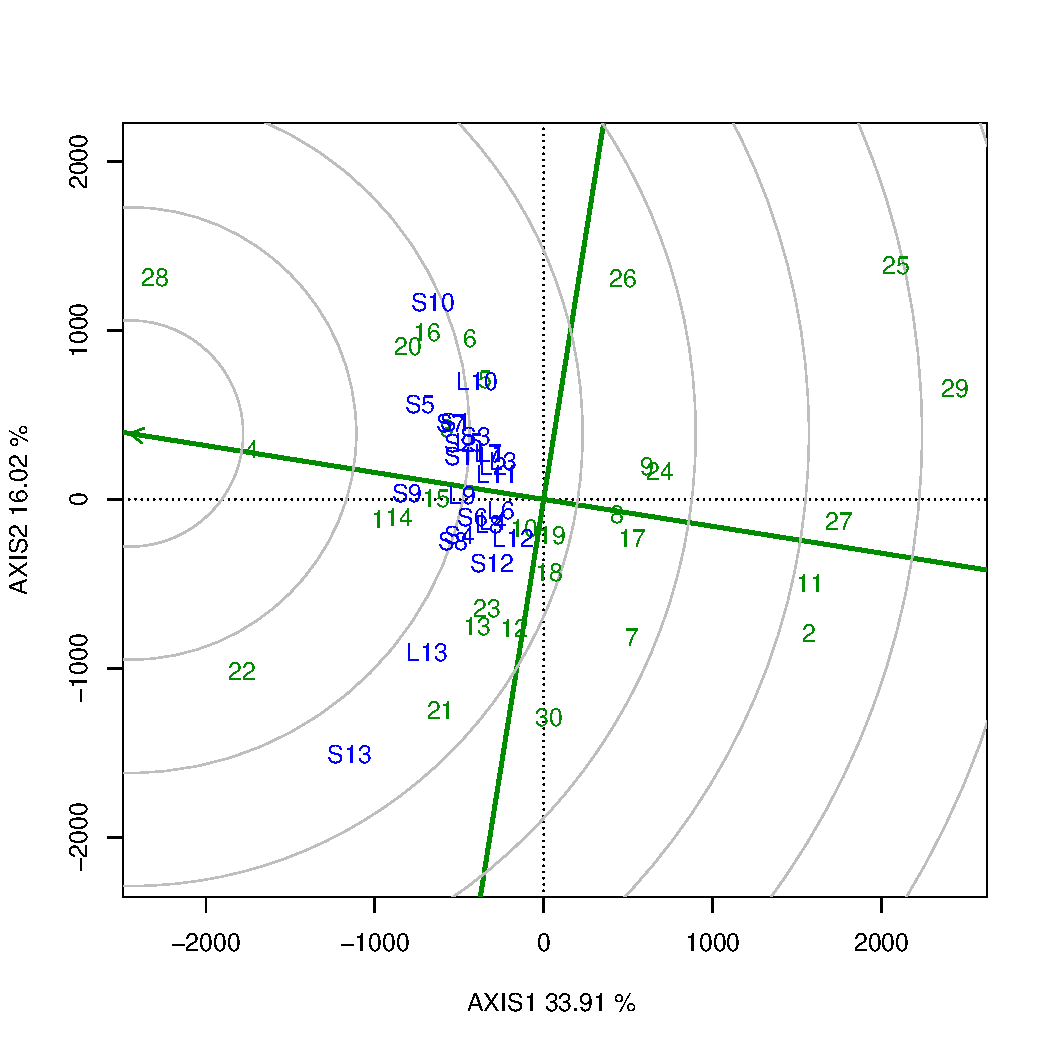
\includegraphics[width=490mm]{02ThesisMain/Ch04RD/figures/idealg}}
	\caption[Comparison of the genotypes with ideal genotype]{GGE-biplot based on genotype-focused scaling for comparison of the genotypes with ideal genotype}
\label{Figure:4.7}
\end{figure}



The ability of environments to discriminate for genotypes are visualized using GGE-biplot presented in concentric circles based on environment focused scaling in [Fig.\ref{Figure:4.8}] . Among environments none of it located at center so not a single environment can be declared ideal. Environment S9(Multan-14) is located at second concentric circle so it may be regarded as favorable environment. Environments  L12(Sargodha), S10(Vehari-14) and S13(Piplan) were distinctly different from other environments. As these environments  were far apart located from center and exhibit low yield potential and are declared as unfavorable environments.

\begin{figure} [H]
	\centering  
	\scalebox{0.3}
	{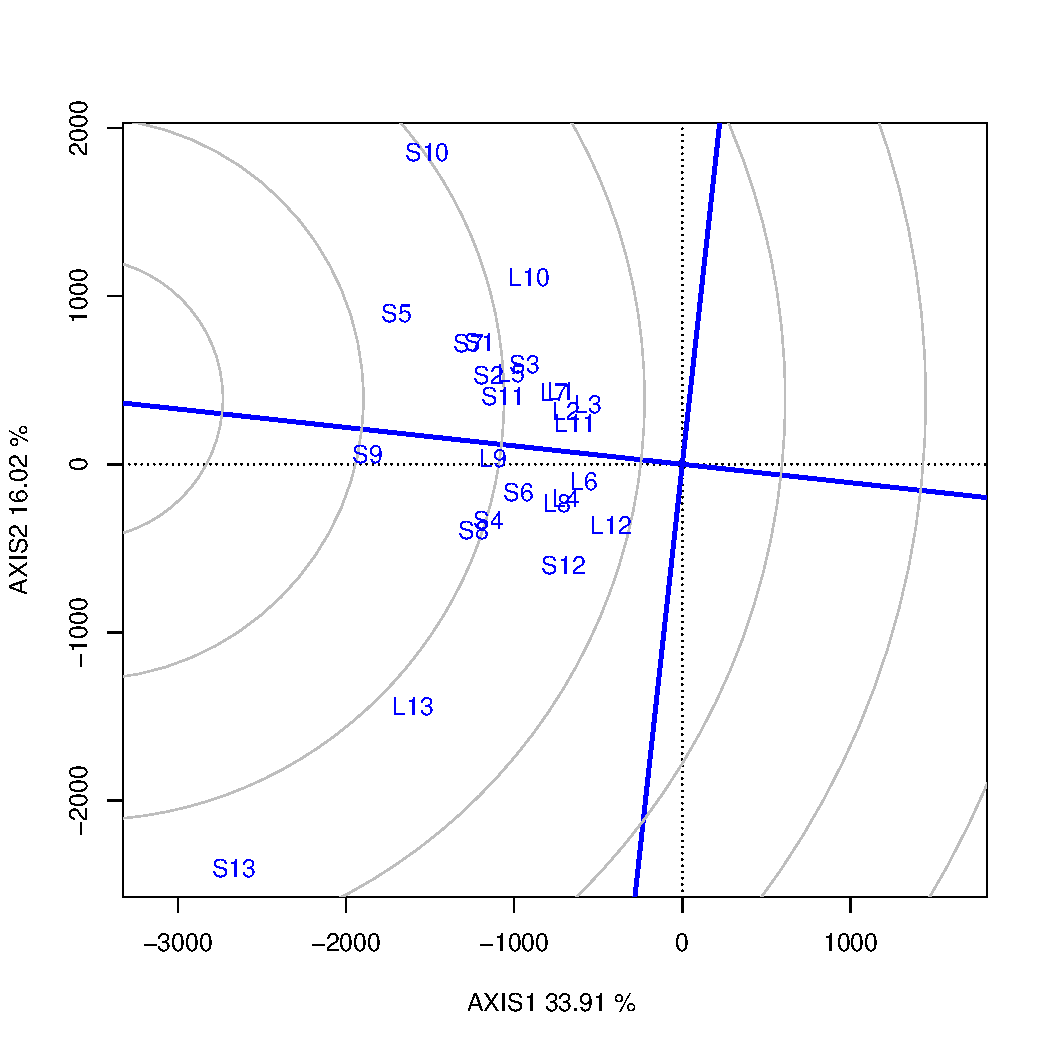
\includegraphics[width=490mm]{02ThesisMain/Ch04RD/figures/idealE}}
	\caption[comparison the environments with ideal environment]{GGE-biplot based on environment-focused scaling for comparison of the environments with ideal environment}
\label{Figure:4.8}
\end{figure}

\subsection{Cluster Analysis}
For assessment of group an similarities among different genotypes, Hierarchical cluster analysis using complete linkage for 30 genotypes was performed using Euclidean distance  given in [Fig.\ref{Figure:4.9}]. Analysis explored that genotypes make small grouping then merge into 3 mega-groups, genotypes V-11098 and Lasani-08 formed a group indicating that these have similarity between them. Similar trends can be observed in other groups   
\begin{figure} [H]
	\centering  
	\scalebox{0.34}
	{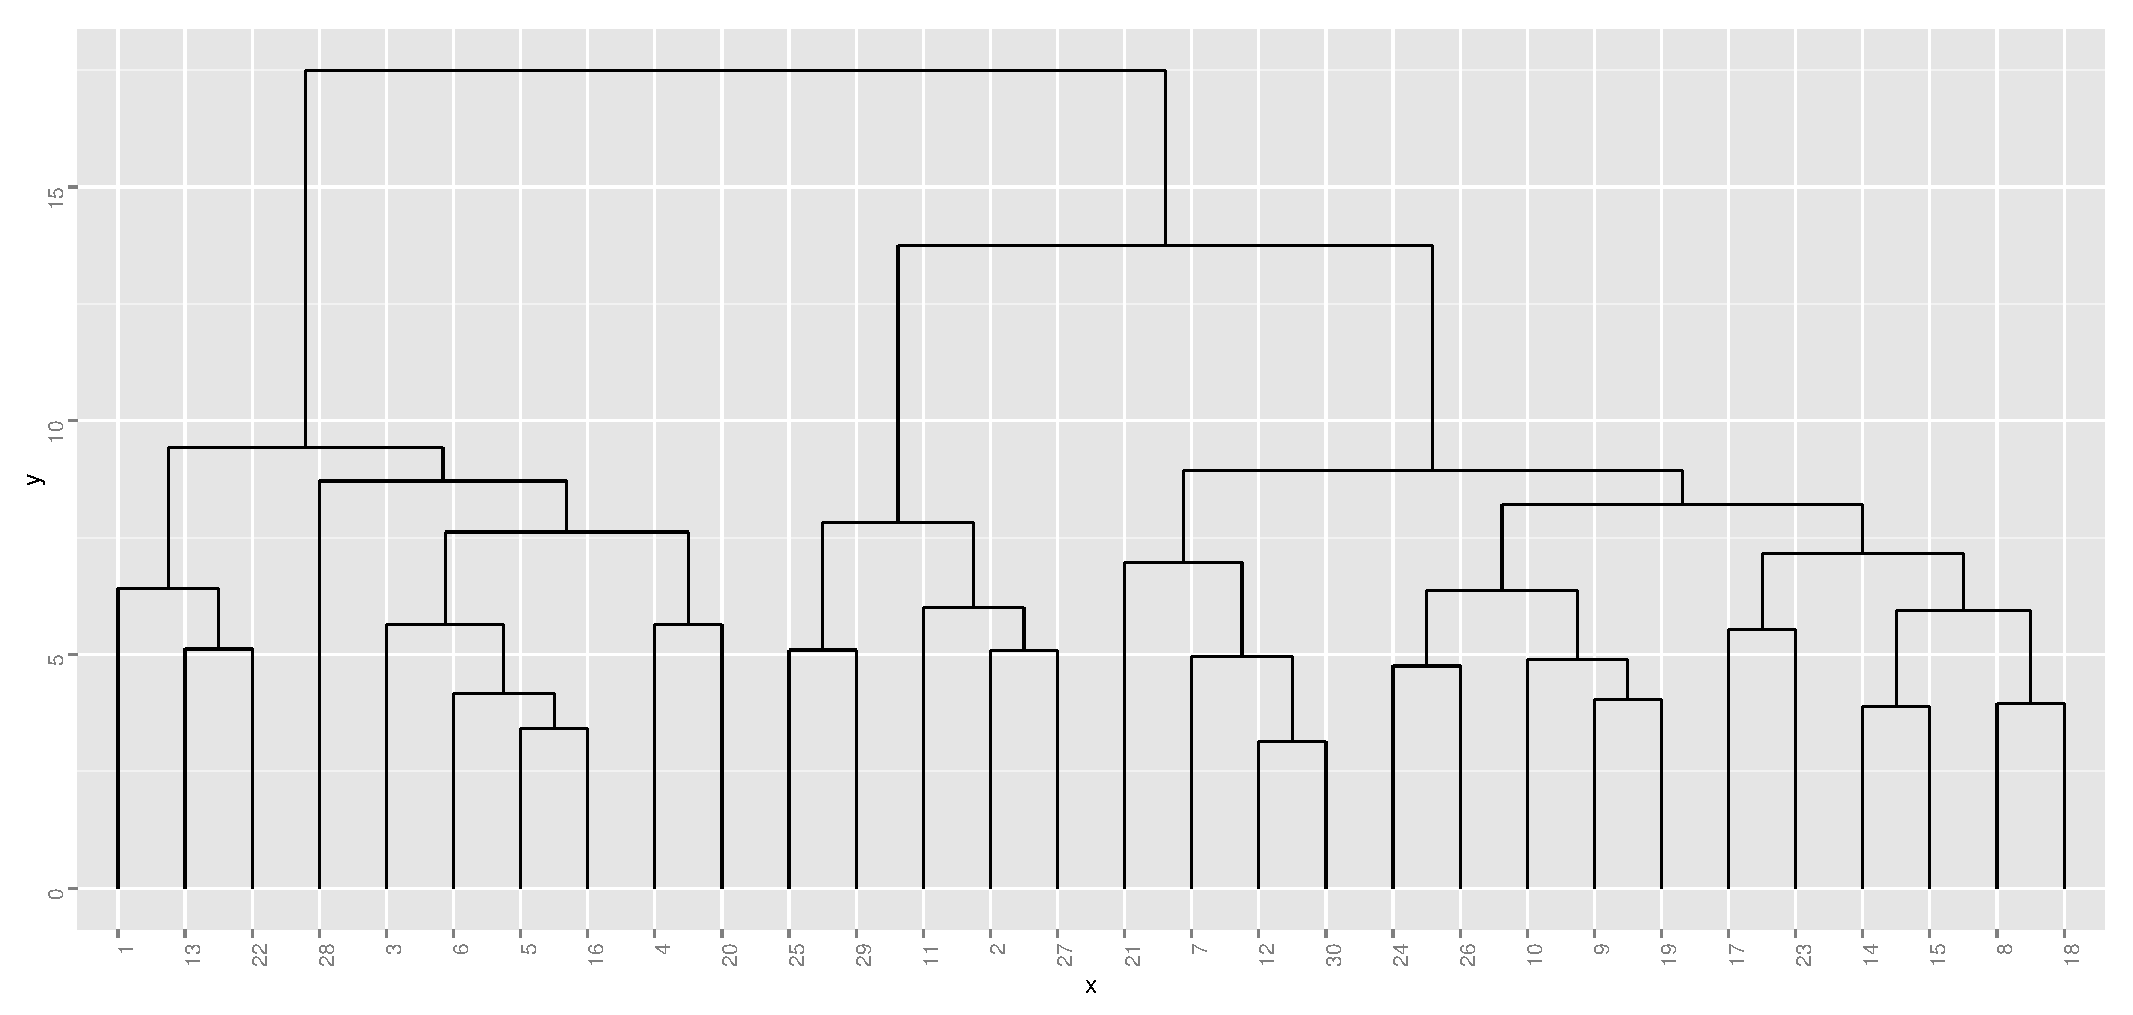
\includegraphics[width=20in,height=20in]{02ThesisMain/Ch04RD/figures/genotype-cluster}}
	\caption[Cluster analysis of genotypes]{Cluster of 30 genotypes for wheat crop data}
\label{Figure:4.9}
\end{figure}


Similarities among environment are assessed by plotting cluster for environments using complete linkage method. From [Fig.\ref{Figure:4.10}] given below it can be observed that environment are divided into four major groups. Environment S13(Piplan-14) form group with S8(Khanewal-14), S9(Multan-14) and S10( Vehari-14). It is noticeable that S6(Gujranwala-14) form group with all environments of year 2013.
\begin{figure} [H]
	\centering  
	\scalebox{0.34}
	{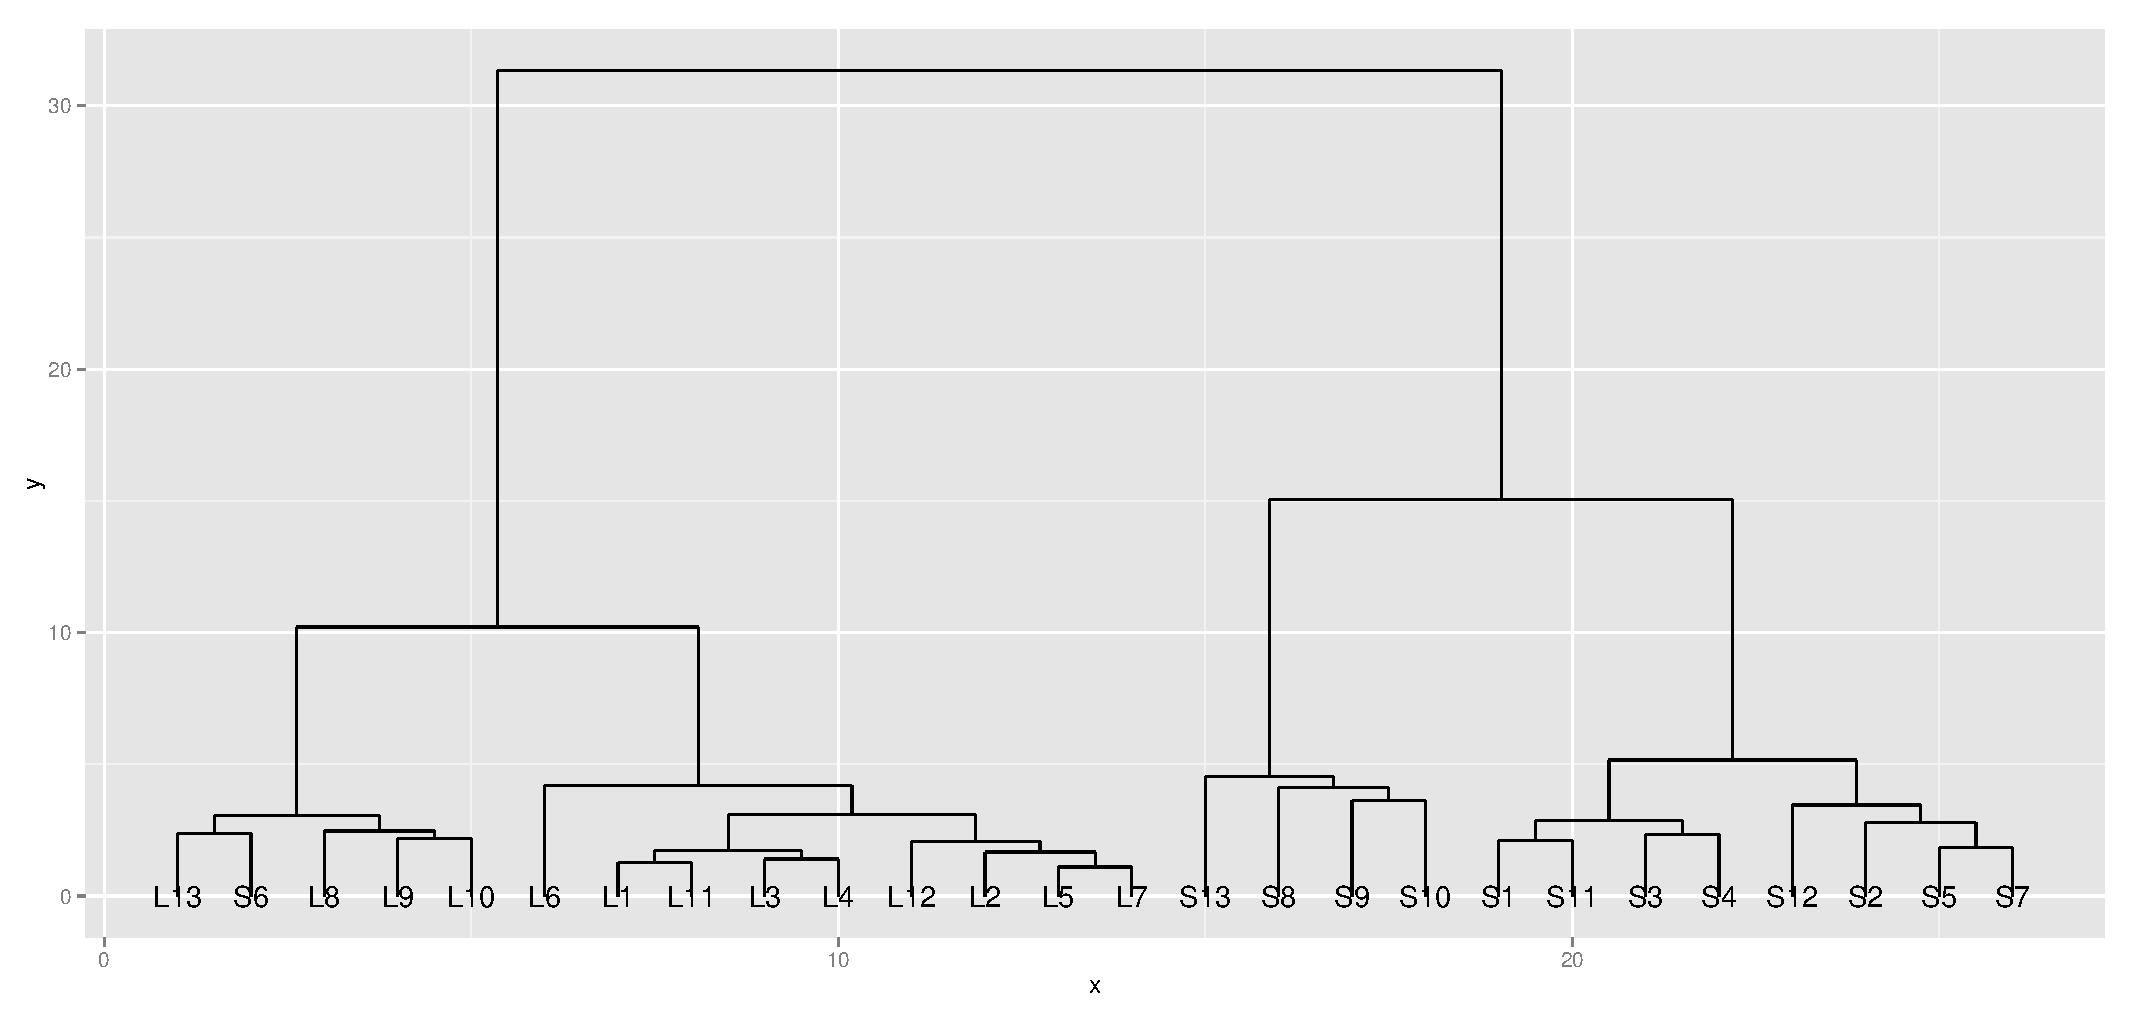
\includegraphics[width=20in,height=20in]{02ThesisMain/Ch04RD/figures/environment-cluster}}
	\caption[Cluster analysis of environments]{Cluster of 13 environments for wheat crop data}
\label{Figure:4.10}
\end{figure}


\section{Bayesian analysis}
A multi-environmental data of two consecutive years was used for analysis which consist of 30 genotypes of wheat crop evaluated in 13 different environments. The layout of experiment was RCBD with three replication for all genotypes as well as for years. To elicit prior, first year data was used and Von-MISES Fisher distribution was applied as proper prior suggested by \citep{PEREZ-ELIZALDE2011}.

 After obtaining large MCMC sample using joint posterior distribution, parametrs were estimated using sample mean. Histogram and traces of $\mu$ and first two singular values ($\lambda_1$,$\lambda_2$) are presented in [Fig.\ref{Figure:4.11}]. These trace and histogram exhibit  that all were slightly positively bell shaped and have acceptable shape with marginal posterior distribution. The Bayesian AMMI estimate for $\lambda_1$ was (2077.26) and for $\lambda_2$ was $1292.73$ and standard deviation for $\lambda_1$ and $\lambda_2$ were 423.2 and 381.9, respectively.The posterior densities of remaining singular values show a tendency to move toward zero, complete posterior densities for singular values are given in (Table~\ref{Table:4.6}).

The histogram of MCMC sample along with marginal posterior singular values ($\lambda_{11}$-$\lambda_{12}$) are shown in [Fig.\ref{Figure:4.12}]. The figure shows a similar pattern first 2,3  posterior singular values have slightly positive bell shape, where as later values tend to have a direction towards zero. Cumulative proportion of variation for posterior densities by eigenvalues explored that about 90\% interaction variance can be explained by four components [Fig.\ref{Figure:4.12}]. It can be evaluated that first component explain about 60\% interaction variation, and second component approximately 17\%. It shows that  two bilinear term can retained in the model as  first two singular values can explain 80\% cumulative variation.  These results of two significant bilinear components are an evidence  with those normally present in the analyses of genotype by environment trials where the requirement  is to have more than one bilinear term in the model to  handle complexity of the G$\times$E \citep{PEREZ-ELIZALDE2011}.

\begin{figure}
	\subfloat[fig 1]{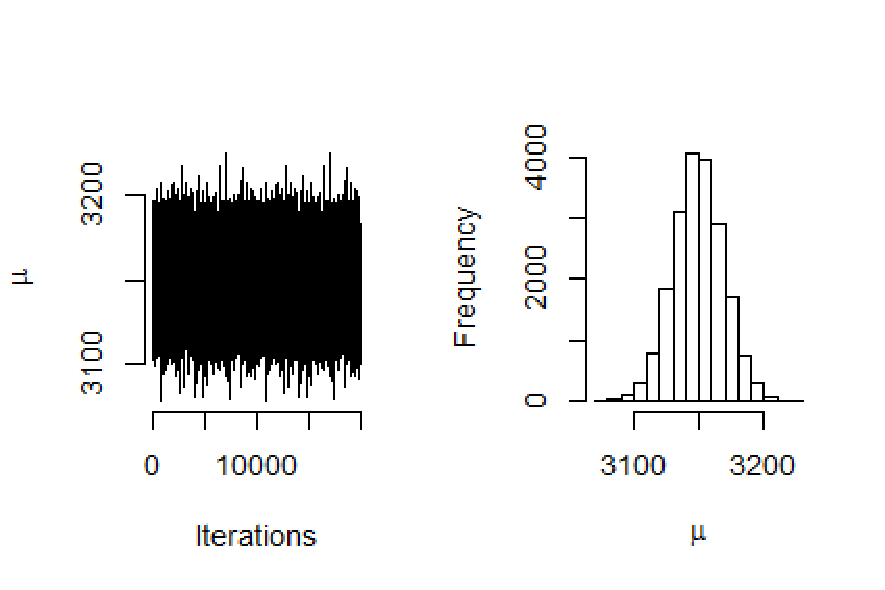
\includegraphics[width = 4in]{02ThesisMain/Ch04RD/figures/tracemu.pdf}} \\
	\subfloat[fig 2]{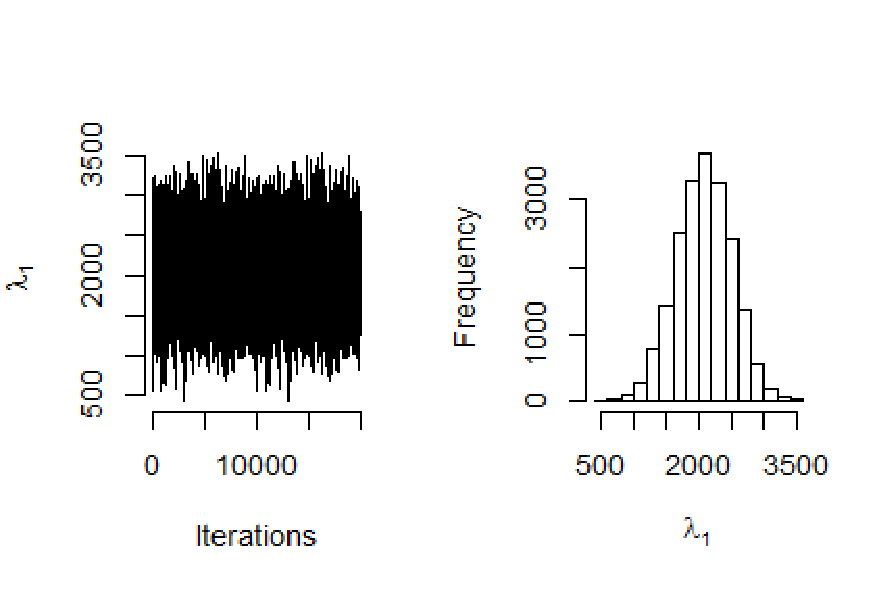
\includegraphics[width = 4in]{02ThesisMain/Ch04RD/figures/tracelambda1.pdf}} \\   
	\subfloat[fig 3]{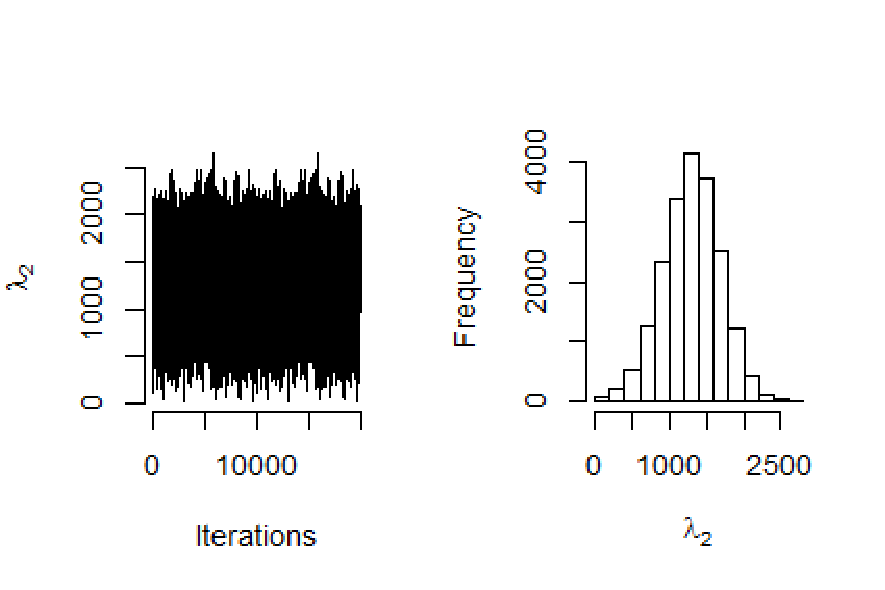
\includegraphics[width = 4in]{02ThesisMain/Ch04RD/figures/tracelambda2.pdf}}
	
	\caption[Trace for MCMC samples]{Traces and histogram of mean and values $\lambda_1$ and $\lambda_2$ obtained from MCMC wheat data}
\label{Figure:4.11}	
\end{figure}



\begin{figure}
	\centering	
	\subfloat[fig 1]{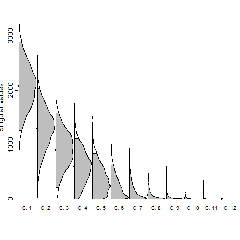
\includegraphics[width = 4in]{02ThesisMain/Ch04RD/figures/screeplot.pdf}} \\
	\subfloat[fig 2]{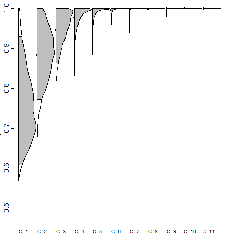
\includegraphics[width = 4in]{02ThesisMain/Ch04RD/figures/cumvar.pdf}}    
	\caption[Posterior densities and regions for singular values and cumulative proportion]{Wheat Crop data of 30 genotypes in 13 environments:(a) Posterior densities and 0.95 HPD regions of the singular values, $\lambda_1,...,\lambda_{11}$ (C.1-C.12); (b) posterior densities and 0.95 HPD regions of the cumulative proportion of variance $\phi_t=\frac{\sum_{k=1}^t\lambda_k^2}{\sum_{k=1}^{min(r,c-1)}\lambda_k^2}$, t = 1,...,min(r, c)-2. }
\label{Figure:4.12}
\end{figure}


\subsection{Uncertainty and confidence regions of first two bilinear terms in Bayesian AMMI}
In general, the values of first bilinear terms $u_{i1}$ and $v_{j1}$ were, either positive or negative, larger than the values than those of other bilinear terms such as of $u_{i2}$ and $v_{j2}$ for mean , whereas the standard deviations (SD) exhibit different pattern as SD, for $u_{i1}$ and $v_{j1}$ were lower than those of $u_{i2}$ and $v_{j2}$ . Further more, HPD regions have narrow length for the first bilinear components of genotypes and environments ($u_{i1}$ and $v_{j1}$) as compared to  the second bilinear components, $u_{i2}$ and $v_{j2}$ [see appendix] . These results are indication that discrimination of genotypes and environment is done more precisely by first bilinear component than those of second bi-leaner component. In general, this is similarity with the classical approach named Principal component analysis (PCA) where the variability explained by first component is alway more than second principal component. The summary is, there was less uncertainty in first bilinear component than second bilinear component.

\subsection{Credible intervals for genotypes}
The posterior, mean, SD and HPD intervals for probability 0.90 and 0.95 are provided in (Table~\ref{Table:4.4}). The posterior Sd of main effects $\alpha_i$ have range from 100.34 t0 103.26.
In general, the values of ui1 and vj1 were, in absolute terms, larger than the values
of ui2 and vj2, whereas the standard deviations (SD) of ui1 and vj1 were smaller than
those of ui2 and vj2. Consequently, the lengths of the HPD regions were narrower for the
first bilinear components of genotypes and environments (ui1 and vj1) than for the second
bilinear components, ui2 and vj2 (data not shown). In summary, there is more posterior
uncertainty in the second bilinear components for genotypes and sites than in the first
bilinear components. Further illustration is provided in (Table~\ref{Table:4.4}).
\begin{table}[h!]
	\centering
	\caption[HPD table for genotypes]{Posterior summary (Mean), standard deviation (SD), quartiles ($q_{0.25}$, $q_{0.50}$, and $q_{0.75}$), 0.90 HPD,  and 0.95 HPD intervals computed with 20,000 approximately independent samples simulated from the posterior distribution of 30 linear effects of genotype for wheat crop data}
	\label{Table:4.4}
	\begin{tabular}{l r r r r r r r r r} 
		\toprule
		&&&&	&&\multicolumn{2}{r}{.90 HPD interval} 
		&\multicolumn{2}{c}{ .95 HPD interval}  \\
		\cmidrule(r){7-8}  \cmidrule(lr){9-10} 
		Para & Mean & SD & $q_{0.25}$ &$q_{0.50}$ & $q_{0.75}$ & lower & Upper & lower & upper\\
		\midrule
		$\mu$       & 3149.47&	19.11 &	3136.41	& 3149.33 &	3162.22 & 3117.90 & 3180.29& 3112.91& 3187.78  \\
		$\alpha_1$  & 144.47 & 102.01 &	76.88   & 144.77  &	213.02	& -24.99  &	308.58 &-48.61  & 350.92\\
		$\alpha_2$  & -299.67& 102.29 &-368.71  &-300.44  &-230.39  &-468.43  &	-132.72&-491.40 & -93.06\\
		$\alpha_3$  &  80.48 & 100.34 &	12.61   & 80.22   &	147.79  &-87.77	  & 241.36 &-113.71 & 280.58\\
		$\alpha_4$	& 343.76 & 101.80 &	274.76	& 343.74  &	411.53	& 184.22  &	519.40 & 145.95 & 543.93 \\
		$\alpha_5$	& 68.06  & 102.55 &-0.988	& 68.10	  & 138.96  &-93.04   &	240.88 & 133.03	& 264.83 \\
		$\alpha_6$	& 111.16 & 101.75 & 42.36	& 111.66  &	179.85  &-55.01   &	278.38 &-91.35  & 305.81 \\
		$\alpha_7$	&-116.49 & 102.68 &-185.74  &-117.63  &-47.77   &-278.46  &	61.121 &-311.26 & 91.21 \\
		$\alpha_8$	&-89.62  & 102.16 &-159.11  &-90.23   &-21.23   &-254.75  &	79.31  &-285.64 & 113.89\\
		$\alpha_9$	&-127.20 & 101.35 &	-196.58 &-127.14  &	-57.99  &-292.96  &	37.66  &-332.64 & 63.68\\
		$\alpha_{10}$&-2.16  & 102.30 &-69.51   &-2.22    &	65.91   &-169.02  &	164.47 &-211.16 & 190.67\\
		$\alpha_{11}$&-296.26& 101.48 &-365.17  &-296.33  &-228.84  &-468.71  &-136.58 &-490.76 &-97.13\\
		$\alpha_{12}$& 6.65  & 101.60 &-61.12   & 7.11    &	75.31   &-163.21  & 171.12 &-195.24 &	204.97\\
		$\alpha_{13}$& 82.29 & 102.6  &	13.19   & 81.11   &	151.35  &-87.60   &	250.91 &-117.20 & 282.40 \\
		$\alpha_{14}$& 161.84& 103.42 &	93.04   & 162.78  & 230.93  &-3.26    & 336.82 &-40.87  & 360.99\\
		$\alpha_{15}$& 114.64& 101.61 &	46.99   & 115.30  &	182.10  &-52.28   & 285.2  &-87.42  & 311.87\\
		$\alpha_{16}$& 125.49& 101.25 & 58.68	& 124.24  & 193.01  &-32.91   &	300.62 &-65.19  & 330.20\\
		$\alpha_{17}$&-64.89 & 101.89 &-134.56  &-65.52   &	4.5839  &-224.59  &	108.64 &-262.62 & 132.10\\
		$\alpha_{18}$&-12.88 & 103.60 &-83.14   &-12.94   &	56.77	&-181.72  & 154.50 &-216.43 & 190.61\\
		$\alpha_{19}$&-29.45 & 102.42 &-99.18   &-29.20   &	40.05	&-200.18  &	134.87 &-244.40 &	156.10\\
		$\alpha_{20}$& 227.33& 100.42 &	160.09  & 227.98  & 295.82  & 69.60   &	396.76 & 31.49  &	424.60\\
		$\alpha_{21}$& 112.95& 102.55 &	43.99   & 112.25  &	181.99  & 50.03	  & 286.92 &-86.49  &	312.11 \\
		$\alpha_{22}$& 252.68& 102.25 & 182.49  & 253.66  &	322.34  & 93.08   &	426.27 & 49.43  & 447.91\\
		$\alpha_{23}$& 32.70 & 102.92 &-36.10   & 31.65   &	102.47	&-136.018 &	199.39 &-167.03 & 233.40\\
		$\alpha_{24}$&-118.83& 102.53 &-187.85  &-119.65  &-49.46 	&-285.57  &	52.50  &-318.81 & 81.03\\
		$\alpha_{25}$&-311.46& 102.30 &-380.53	&-310.35  &-243.37 	&-482.56  &-145.76 &-507.53 &-109.09\\
		$\alpha_{26}$&-35.89 & 102.61 &-105.44  &-36.89   & 33.58 	&-197.72  &	138.63 &-245.10 &	156.20\\
		$\alpha_{27}$&-340.15& 101.36 &-408.19  &-339.38  &	-270.92 &-502.16  &	-168.85&-536.61	&-141.80\\
		$\alpha_{28}$& 441.91& 102.22 &	374.73  & 442.90  &	511.35  & 276.88  & 612.36 & 243.23 &	648.14\\
		$\alpha_{29}$&-429.16& 103.26 &-498.31  &-428.42  &-359.38  &-602.33  & -262.07&-628.11 & -222.16\\
		$\alpha_{30}$&-32.3  & 101.5  &-100.46  &-31.99   &36.55    &-201.45  &	131.06 &-227.45 &	171.49\\
		
		\bottomrule
	\end{tabular}
\end{table} 




\subsection{Credible intervals for environments}
The posterior, mean, SD and HPD intervals for probability .90 and .95 for environment main effect are provided in (Table~\ref{Table:4.6}). The posterior SD of main effects $\beta_j$ have range from 64.80 t0 66.36.
\begin{table}[h!]
	\centering
	\caption[HPD table for environments]{Posterior summary (Mean), standard deviation (SD), quartiles ($q_{0.25}$, $q_{0.50}$, and $q_{0.75}$), 0.90 HPD, and 0.95 HPD intervals computed with 20,000 approximately independent samples simulated from the posterior distribution of  13 linear effect of environments wheat crop data} 
	\label{Table:4.5}
	\begin{tabular}{l r r r r r r r r r} 
		\toprule
		&&&&& & \multicolumn{2}{c}{.90 HPD Interval} 
		&\multicolumn{2}{c}{ .95 HPD interval}  \\
		\cmidrule(r){7-8}  \cmidrule(lr){9-10} 
		Para & Mean & SD & $q_{0.25}$ &$q_{0.50}$ & $q_{0.75}$ & lower & Upper & lower & upper\\
		\midrule
		
$\beta_1$  & -62.10  & 66.36 & -106.74 &-62.45  & -17.49  &-171.05 & 45.249 &-188.46 & 69.61 \\
$\beta_2$  &-440.83  & 65.57 & -485.00 &-440.82 & -395.33 &-548.69 & -335.02&-567.72 &-312.09\\
$\beta_3$  &-137.94  & 65.52 &-182.41  &-138.00 &-93.69   & -242.82& -28.64 &-275.31 &-18.64\\
$\beta_4$  & 28.50   & 65.90 &-16.00   & 28.62  & 73.100  &	-77.38 & 137.87 &-101.63 & 155.95 \\
$\beta_5$  &-429.95  & 65.85 & -474.58 &-430.60 & -384.73 &	-533.56& -318.72&-558.36 &-303.55\\
$\beta_6$  &-980.62  & 65.59 &-1024.24 &-981.34 & -936.84 &-1084.69&-868.05 &-1104.70&-845.19 \\
$\beta_7$  &-250.62  & 66.00 &-294.87  &-251.14 &-205.93  &-356.828&-140.71 &-383.77 &-126.10 \\
$\beta_8$  & 1028.13 & 65.89 & 983.95  & 1028.66& 1071.78 &	918.98 & 1135.92& 899.01 & 1154.80 \\
$\beta_9$  & 745.15	 & 65.72 & 700.67  & 745.42 & 789.45  &	634.47 & 849.65 & 616.27 & 871.52 \\
$\beta_{10}$& 600.14 & 66.03 & 556.00  & 600.40 & 644.77  &	494.81 & 711.38 & 465.49 & 725.05 \\
$\beta_{11}$&-131.97 & 65.28 &-176.06  & -131.55& -88.76  &-236.91 &-22.04  &-261.44 &-4.74  \\
$\beta_{12}$&-539.01 & 65.08 &-581.73  &-539.37 & -496.44 &	-650.78&-434.14 &-662.55 &-406.02 \\
$\beta_{13}$& 571.13 & 64.80 & 527.11  & 570.95 & 614.77  &	464.81 & 677.83 & 444.81 & 696.26 \\
		\bottomrule
	\end{tabular}
\end{table} 








\subsection{Credible Regions of the First Two Bilinear Terms of the Linear Bilinear
	Model}
The bilinear terms which do not include the null point (0, 0) for the bivariate 0.90 and .95  HPD region are referred as significant terms, it mean these terms significantly contribute in explanation of interaction variation \citep{PEREZ-ELIZALDE2011}.

In (Table~\ref{Table:4.6}) the posterior mean of 12 singular values and their .95 and .90 Highest posterior density (HPD) are give. It can be seen that the first two eigenvalues have high value where as remaining values tends to moves towards zero. Along with singular values, eigenvectors values for those genotypes and environments are give which do not have null points for .90 HPD and .95 HPD. The score of environment S13 ($v_{13,1}$) and genotype 25 ($u_{25,1}$) score do not have null point for both HPD intervals, indicates that they have significant contribution in G $\times$ E.  
\begin{table}[h!]
	\centering
	\caption[HPD table for significant bilinear components]{Posterior summary (Mean), standard deviation (SD), quartiles ($q_{0.25}$, $q_{0.50}$, and $q_{0.75}$), 0.90 HPD, and 0.95 HPD intervals computed with 20,000 approximately independent samples simulated from the posterior distribution of the residual variance ($\sigma$ ), all singular values $(\lambda_1, . . . , \lambda_{12})$ and the right and
		the left singular vector elements of genotypes and environments, respectively, whose 0.90 HPD and
		0.95 HPD intervals do not contain the null value (0, 0). Data for wheat yield} 
\label{Table:4.6}
	\begin{tabular}{l r r r r r r r r r} 
		\toprule
		&&&&&& \multicolumn{2}{c}{.90 HPD Interval}  
		&\multicolumn{2}{c}{ .95 HPD interval}  \\
		\cmidrule(r){7-8}  \cmidrule(lr){9-10} 
		Para & Mean & SD & $q_{0.25}$ &$q_{0.50}$ & $q_{0.75}$ & lower & Upper & lower & upper\\
		\midrule
	
$\lambda_1$ & 2077.26& 423.20 & 790.88 & 2084.27 & 2369.18 & 1369.07 & 2748.10 & 1240.48 & 2888.35 \\
$\lambda_2$ & 1292.73& 381.89 & 1036.29& 1303.84 & 1553.56 & 675.14	 & 1920.03 & 533.34  & 2018.84\\
$\lambda_3$ & 903.23 & 347.96 & 664.77 & 909.93  & 1148.50 & 316.96  & 1470.83 & 216.29& 1579.14\\
$\lambda_4$	& 597.50 & 306.67 &	371.38 & 588.14  & 814.40  & 24.49   & 1022.25 & 0.1407  &	1110.15\\
$\lambda_5$	& 379.46 & 254.98 &	173.69 & 348.85  & 556.13  & 0.0037  & 734.44  & 0.0037  &	836.66\\
$\lambda_6$	& 236.08 & 199.88 &	66.70  & 191.74  & 359.06  & 0.0015  & 528.47  & 0.0015  &	621.69\\
$\lambda_7$ & 140.88 & 150.84 &	22.27  & 87.94   & 213.78  & 0.0001  &	365.08 & 0.0001  &	458.43\\
$\lambda_8$ & 79.15  & 106.10 &	6.91   & 34.94   & 109.76  & 0.00    &	225.29 & 0.00    &	314.97\\
$\lambda_9$ & 43.05  & 70.21  &	2.27   & 13.20   & 51.13   & 0.00    &	128.98 & 0.00    & 190.38\\
$\lambda_{10}$& 22.06& 42.92  &	0.71   & 4.81    & 22.37   & 0.00    &	65.143 &  0.00   &	108.12\\
$\lambda_{11}$& 11.51& 26.51  &	0.22   & 1.68    &	9.66   & 0.00    &	31.60  &  0.00   &	58.90 \\
$\lambda_{12}$&	5.88 & 15.83  &	0.073  & 0.62    &	3.94   & 0.00	 & 15.14   & 0.00	 & 30.46 \\
$u_{25_1}$	  & 0.23 & 0.141  & 0.14   & 0.244	 & 0.33	   & 0.015   &	0.47   & -0.041	 & 0.501 \\
$v_{13,1}$    &-0.63 & 0.11   &	-0.71  & -0.64   &-0.55    &-0.81    &	-0.45  & -0.83   &	-0.39 \\
		
		\bottomrule
	\end{tabular}
\end{table} 
\clearpage
Biplot for the bivariate 0.90 HPD and 0.95 HPD regions  of column score is shown in Figure [Fig.\ref{Figure:4.13}]. Visual analysis shown that S10 form a group of distinct group of environment which have positive value, while S13 showed a negative correlation with S10. some degree of similarity was also shown between S13 and S9,  S10 overlap with S12, S8 and S4, it means they form a homogeneous group. whereas, S2, S3, S1, S5, S7 and S11 form a group which were not as significant as others.
\begin{figure} [H]
	\centering  
	\scalebox{0.3}
	{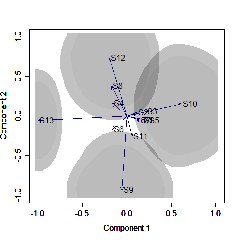
\includegraphics[width=540mm]{02ThesisMain/Ch04RD/figures/c-biplot-80-90.pdf}}
	\caption[Bayesian biplot for environments]{Wheat crop data of 30 genotypes in 13 environments: plot of the bivariate column scores $\textbf{V}^\prime\textbf{D}^{1/2}$ and the bivariate 0.95 (gray external contour) and 0.90 (gray internal contour) HPD regions}
\label{Figure:4.13}
\end{figure}


In [Fig.\ref{Figure:4.14}] bi-plot for row score is shown, among all genotypes 25($u_{25,1}$) was far away  showing positive value, followed by genotypes 20, 29 and 26 overlapping each other show some similarities among them. These genotypes form a distinct group. Genotype 25 is only which do not contain null point (0,0) and significantly contributed to the interaction. The remaining genotypes form an other group in first bilinear components are not different from zero.
\begin{figure} [H]
  
	\scalebox{0.3}
	{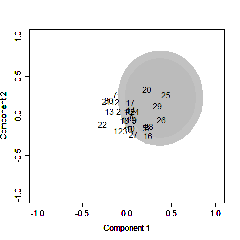
\includegraphics[width=550mm]{02ThesisMain/Ch04RD/figures/r-biplot-80-90.pdf}}
	\caption[Bayesian biplot for genotypes]{Wheat crop data of 30 genotypes in 13 environments: plot of the bivariate row scores $\textbf{U}^\prime\textbf{D}^{1/2}$ and the bivariate 0.95 (gray external contour) and 0.90 (gray internal contour) HPD regions}
\label{Figure:4.14}
\end{figure}


As biplots are based on 0.90 and 0.95 HPD interval have shown overlapping so some significant environment may not be clearly portrayed. A hierarchical clustering based on posterior mean of Euclidean distance between the rows having interaction with complete linkage method was performed [Fig.\ref{Figure:4.15}]. It can be seen that S10 form a single group then merge into other groups, similarly S9 and S13 form a cluster is an evidence that there is some similarity between them.   
\begin{figure} [H]
	\centering  
	\scalebox{0.3}
	{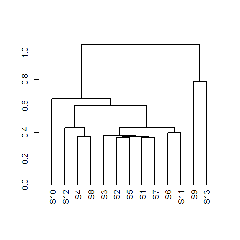
\includegraphics[width=550mm]{02ThesisMain/Ch04RD/figures/column-cluster.pdf}}
	\caption[Bayesian dendrogram for environments]{Dendrogram of the 13 environments using the first two right singular vectors}
\label{Figure:4.15}
\end{figure}


A clusters analysis using posterior mean for genotypes using first two left singular vectors was also performed shown in [Fig.\ref{Figure:4.16}]. Genotypes merge into 4 major clusters, gen-20, gen-29 and gen-25 form a cluster showing these have some similar characteristics among them.This technique for the identification of homogeneous genotypes and environment subsets in is analogous to that provided by \citep{Burguenoa2008}
\begin{figure} [H]
	\centering  
	\scalebox{0.3}
	{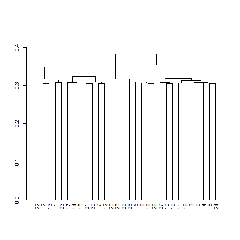
\includegraphics[width=550mm]{02ThesisMain/Ch04RD/figures/row-cluster.pdf}}
	\caption[Bayesian dendrogram for genotpyes]{Dendrogram of the 30 genotypes using the first two left singular vectors}
\label{Figure:4.16}
\end{figure}

 The graphical comparison between the biplots obtained using ordinary least square method (OLS) and Bayesian is given in [Fig.\ref{Figure:4.17}]. Both method provide almost similar results, it is also an indication that Bayesian can be adapted for the analysis of trails which have G$\times$E interaction.   



\begin{figure} [H]
	
	\scalebox{0.32}
	{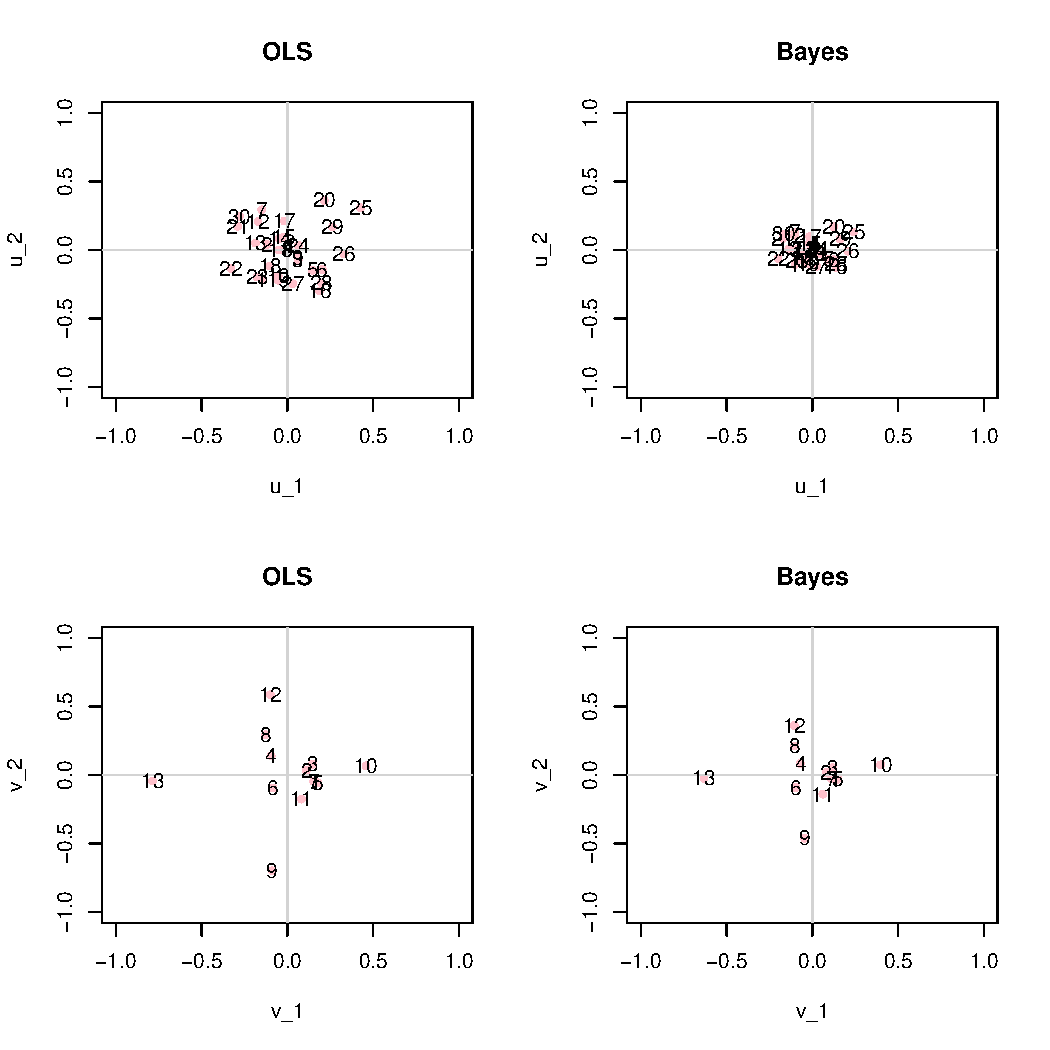
\includegraphics[width=560mm]{02ThesisMain/Ch04RD/figures/comparison.pdf}}
	\caption[Comparison between OLS and Bayes method]{Comparison between the biplots of Classical AMMI using ordinary least square method and Bayesian approach for 30 genoypes and 13 environments of wheat crop data}
\label{Figure:4.17}
\end{figure}


 OLS biplot have more spread-ed observation as compared to Bayesian biplot. Both revealed that genotype 25 and environment 13 (Pilpan) are highly significant and explain the variability of interaction. 
